% Name: Semilog plot
% Description: The error of three iterative solvers against the iteration count on a logarithmic y axis, where linear convergence becomes a straight line whose slope is the rate.
% Tags: semilog, logarithmic axis, convergence, iterative methods

\usepackage{pgfplots}
\pgfplotsset{compat=1.18}

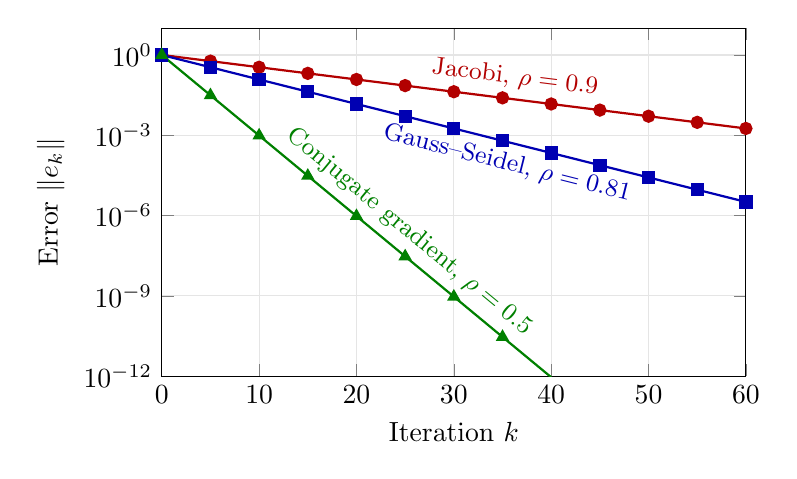
\begin{tikzpicture}
  \begin{semilogyaxis}[
    width=9cm, height=6cm, domain=0:60, samples=13,
    xmin=0, xmax=60, ymin=1e-12, ymax=10,
    xlabel={Iteration $k$}, ylabel={Error $\|e_k\|$},
    ytick={1,1e-3,1e-6,1e-9,1e-12},
    grid=major, grid style={gray!20}, every axis plot/.append style={thick},
  ]
    % Each error is rho^k for the method's convergence rate rho.
    \addplot[red!70!black, mark=*] {0.9^x} node[pos=0.6, sloped, above, font=\small] {Jacobi, $\rho = 0.9$};
    \addplot[blue!70!black, mark=square*] {0.81^x} node[pos=0.6, sloped, below, font=\small] {Gauss--Seidel, $\rho = 0.81$};
    \addplot[green!50!black, mark=triangle*, domain=0:40, samples=9] {0.5^x} node[pos=0.6, sloped, above, font=\small] {Conjugate gradient, $\rho = 0.5$};
  \end{semilogyaxis}
\end{tikzpicture}
